\section{Выполнение, результаты}
Установка съюстирована при помощи микрометрических винтов, отвечающих за фокусировку конденсатора и настройку ширины щели. Настройка проивзодилась на излучении неоновой лампы.

\subsection{Калибровка}
Спектрометр, используемый в работе, требует калибровки, которая была произведена по спектрам излучения неона (длинноволновый диапазон) и ртути (коротковолновый диапазон). Для этого были сопоставлены длины волн табличных линий спектра данных элементов и соответствующие им показания барабана спектрометра (в градусах поворота). Данные можно найти в таблицах 1 и 2 приложения.

По данным построена аппроксимация двумя линейными зависимостями. Рассчитаны коэффициенты методом наименьших квадратов. Соответствующие графики приведены ниже. Инструментальная погрешность каждого измерения достаточно мала и составляла около 2-3 градусов оборота барабана. Дисперсионная, случайная погрешность:
$$\sigma = \sqrt{\frac{\sum_{i = 1}^n(x_i - <x>)^2}{n - 1}} \approx 220A,$$
что соответствует примерно 4\%. 

\begin{figure}[H]
    \centering
    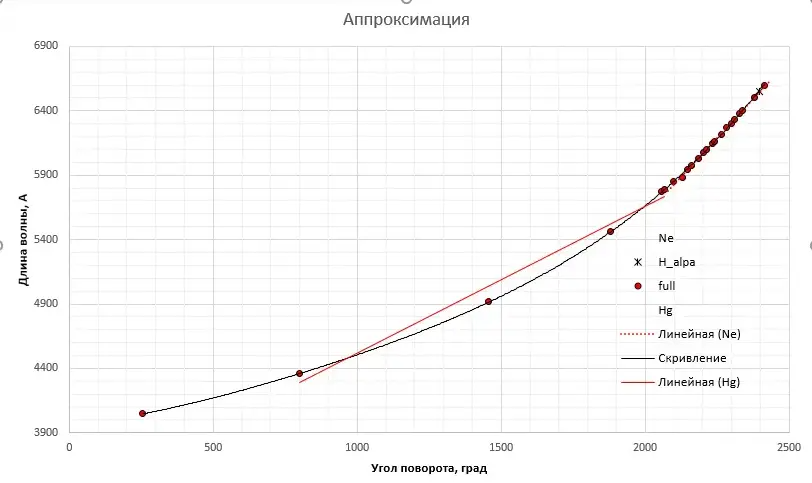
\includegraphics[width=0.9\textwidth]{img/full.png}
    \caption{Полная зависимость, аппроксимация}
    \label{fig:Ne}
\end{figure}

\begin{figure}[H]
    \centering
    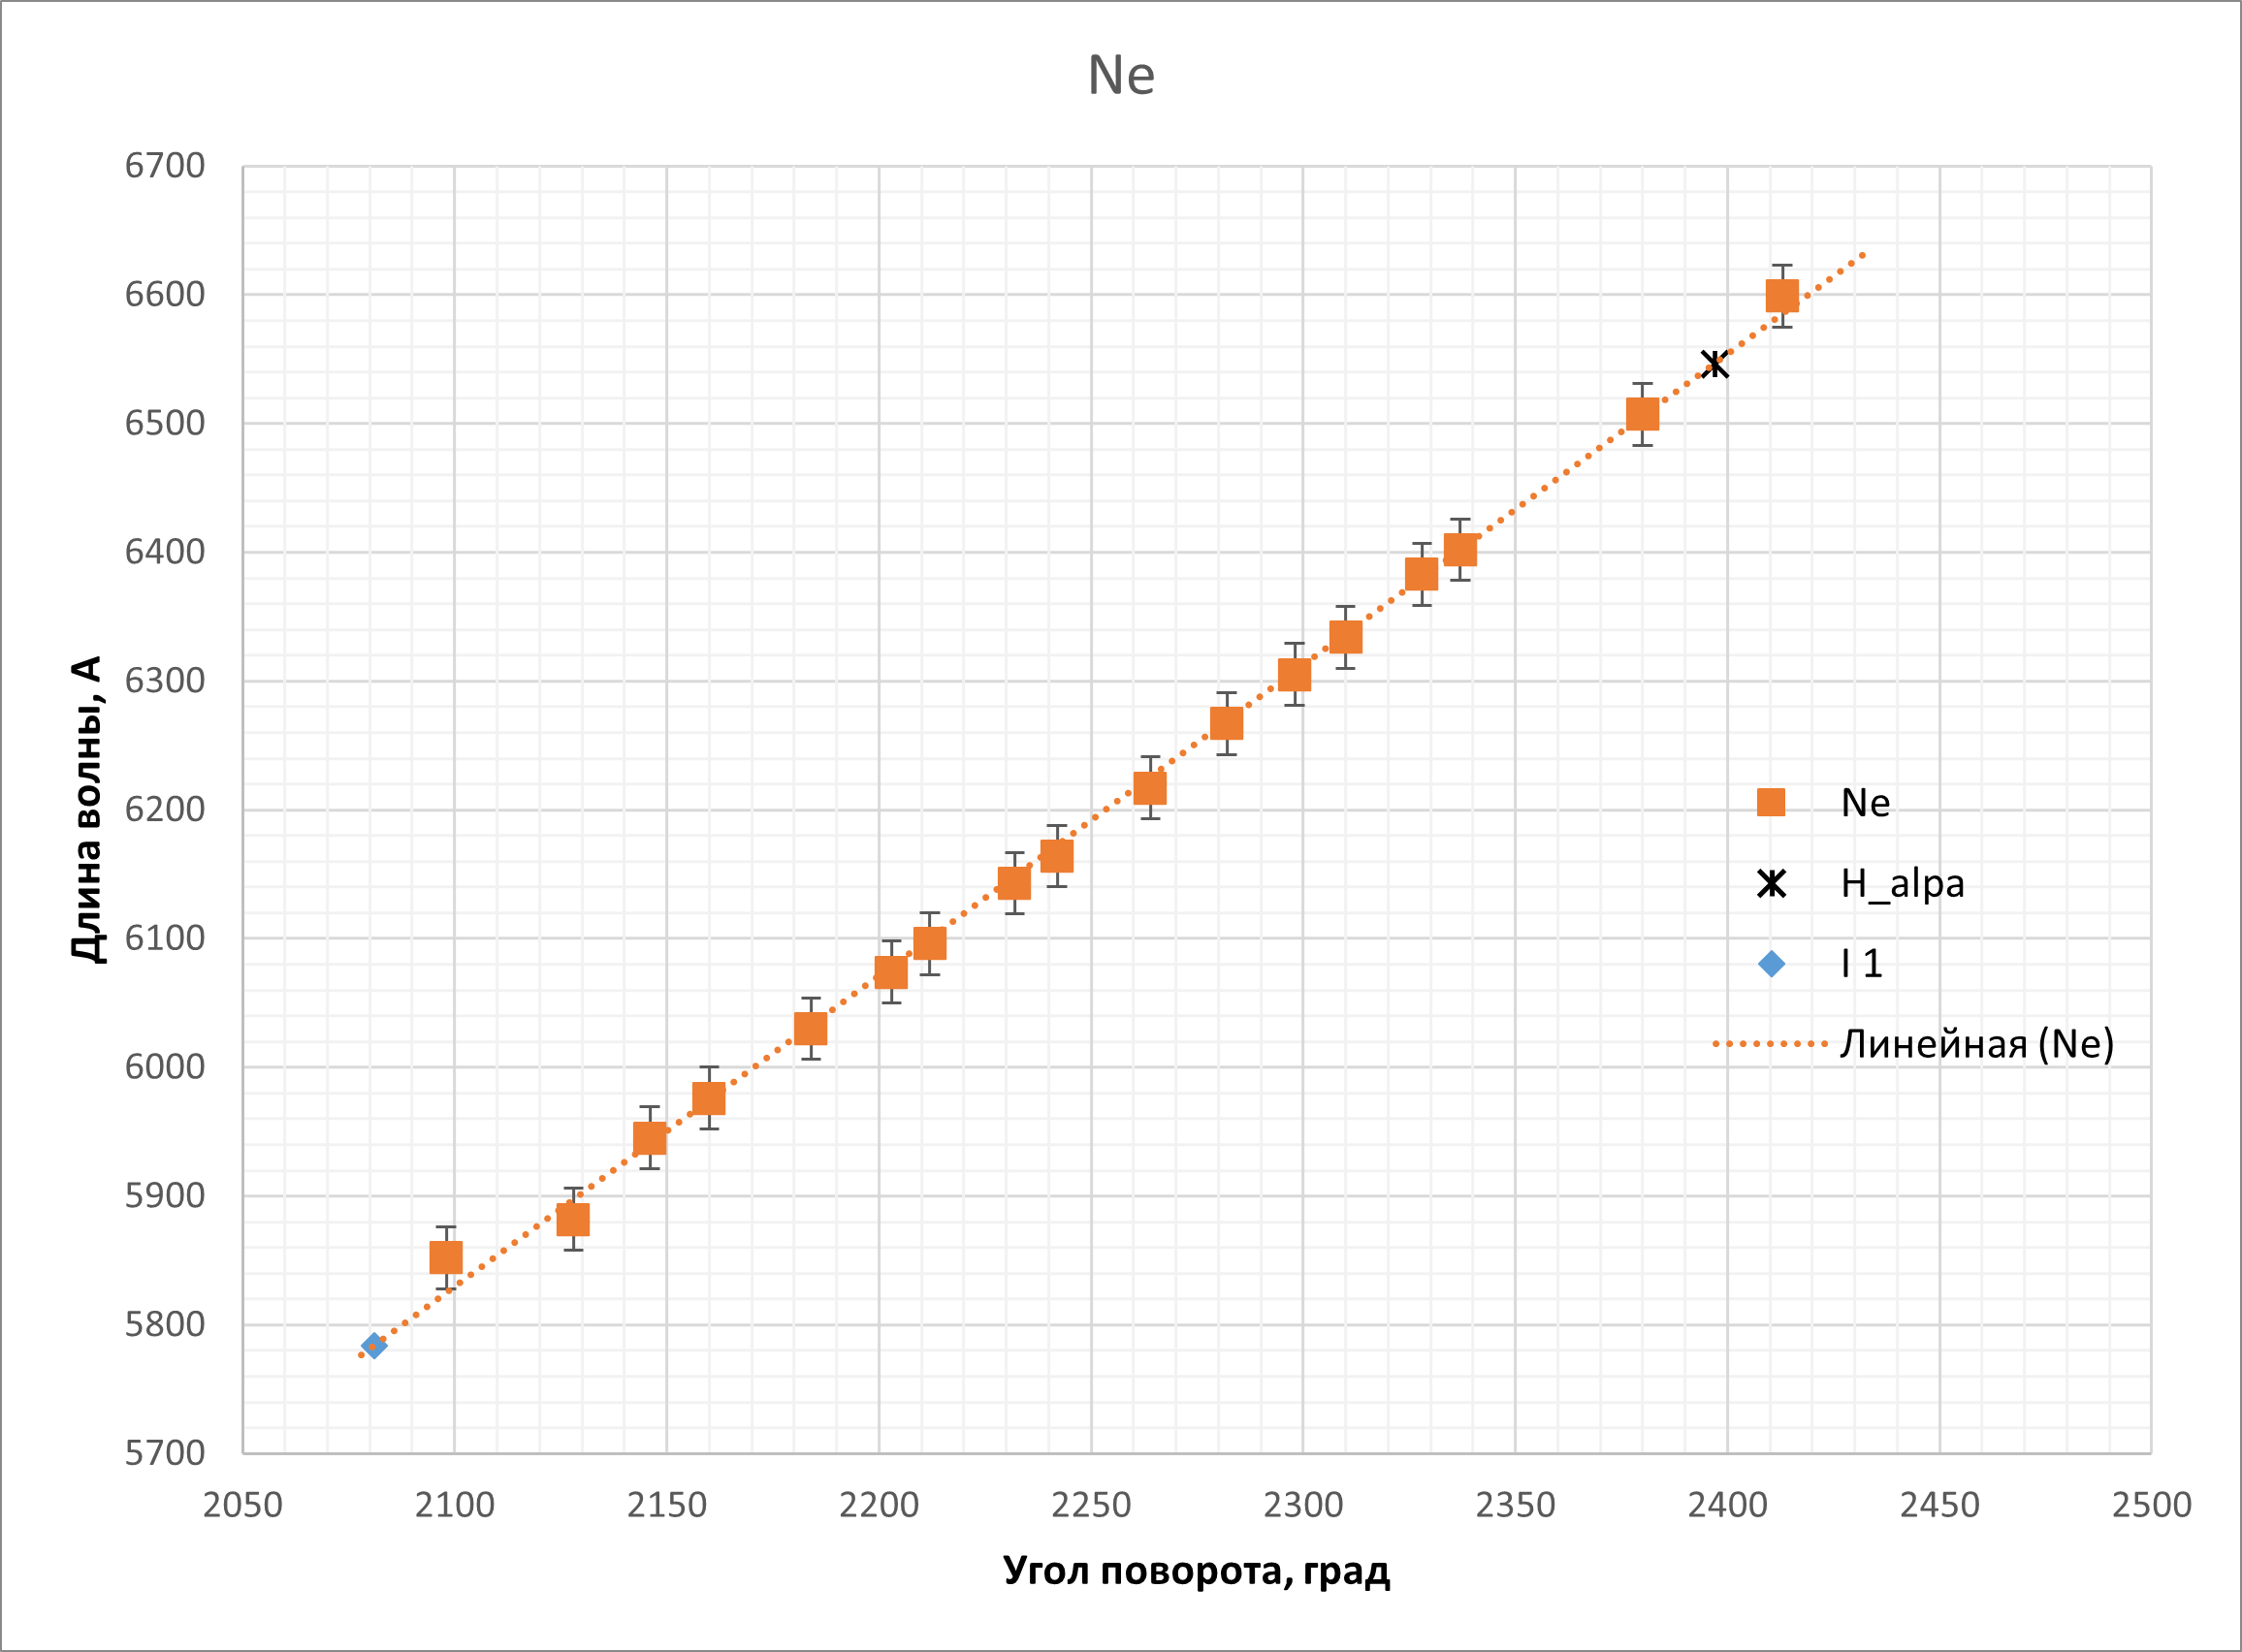
\includegraphics[width=0.7\textwidth]{img/NePlot.png}
    \caption{Калибровка на Ne}
    \label{fig:Ne}
\end{figure}

\begin{figure}[H]
    \centering
    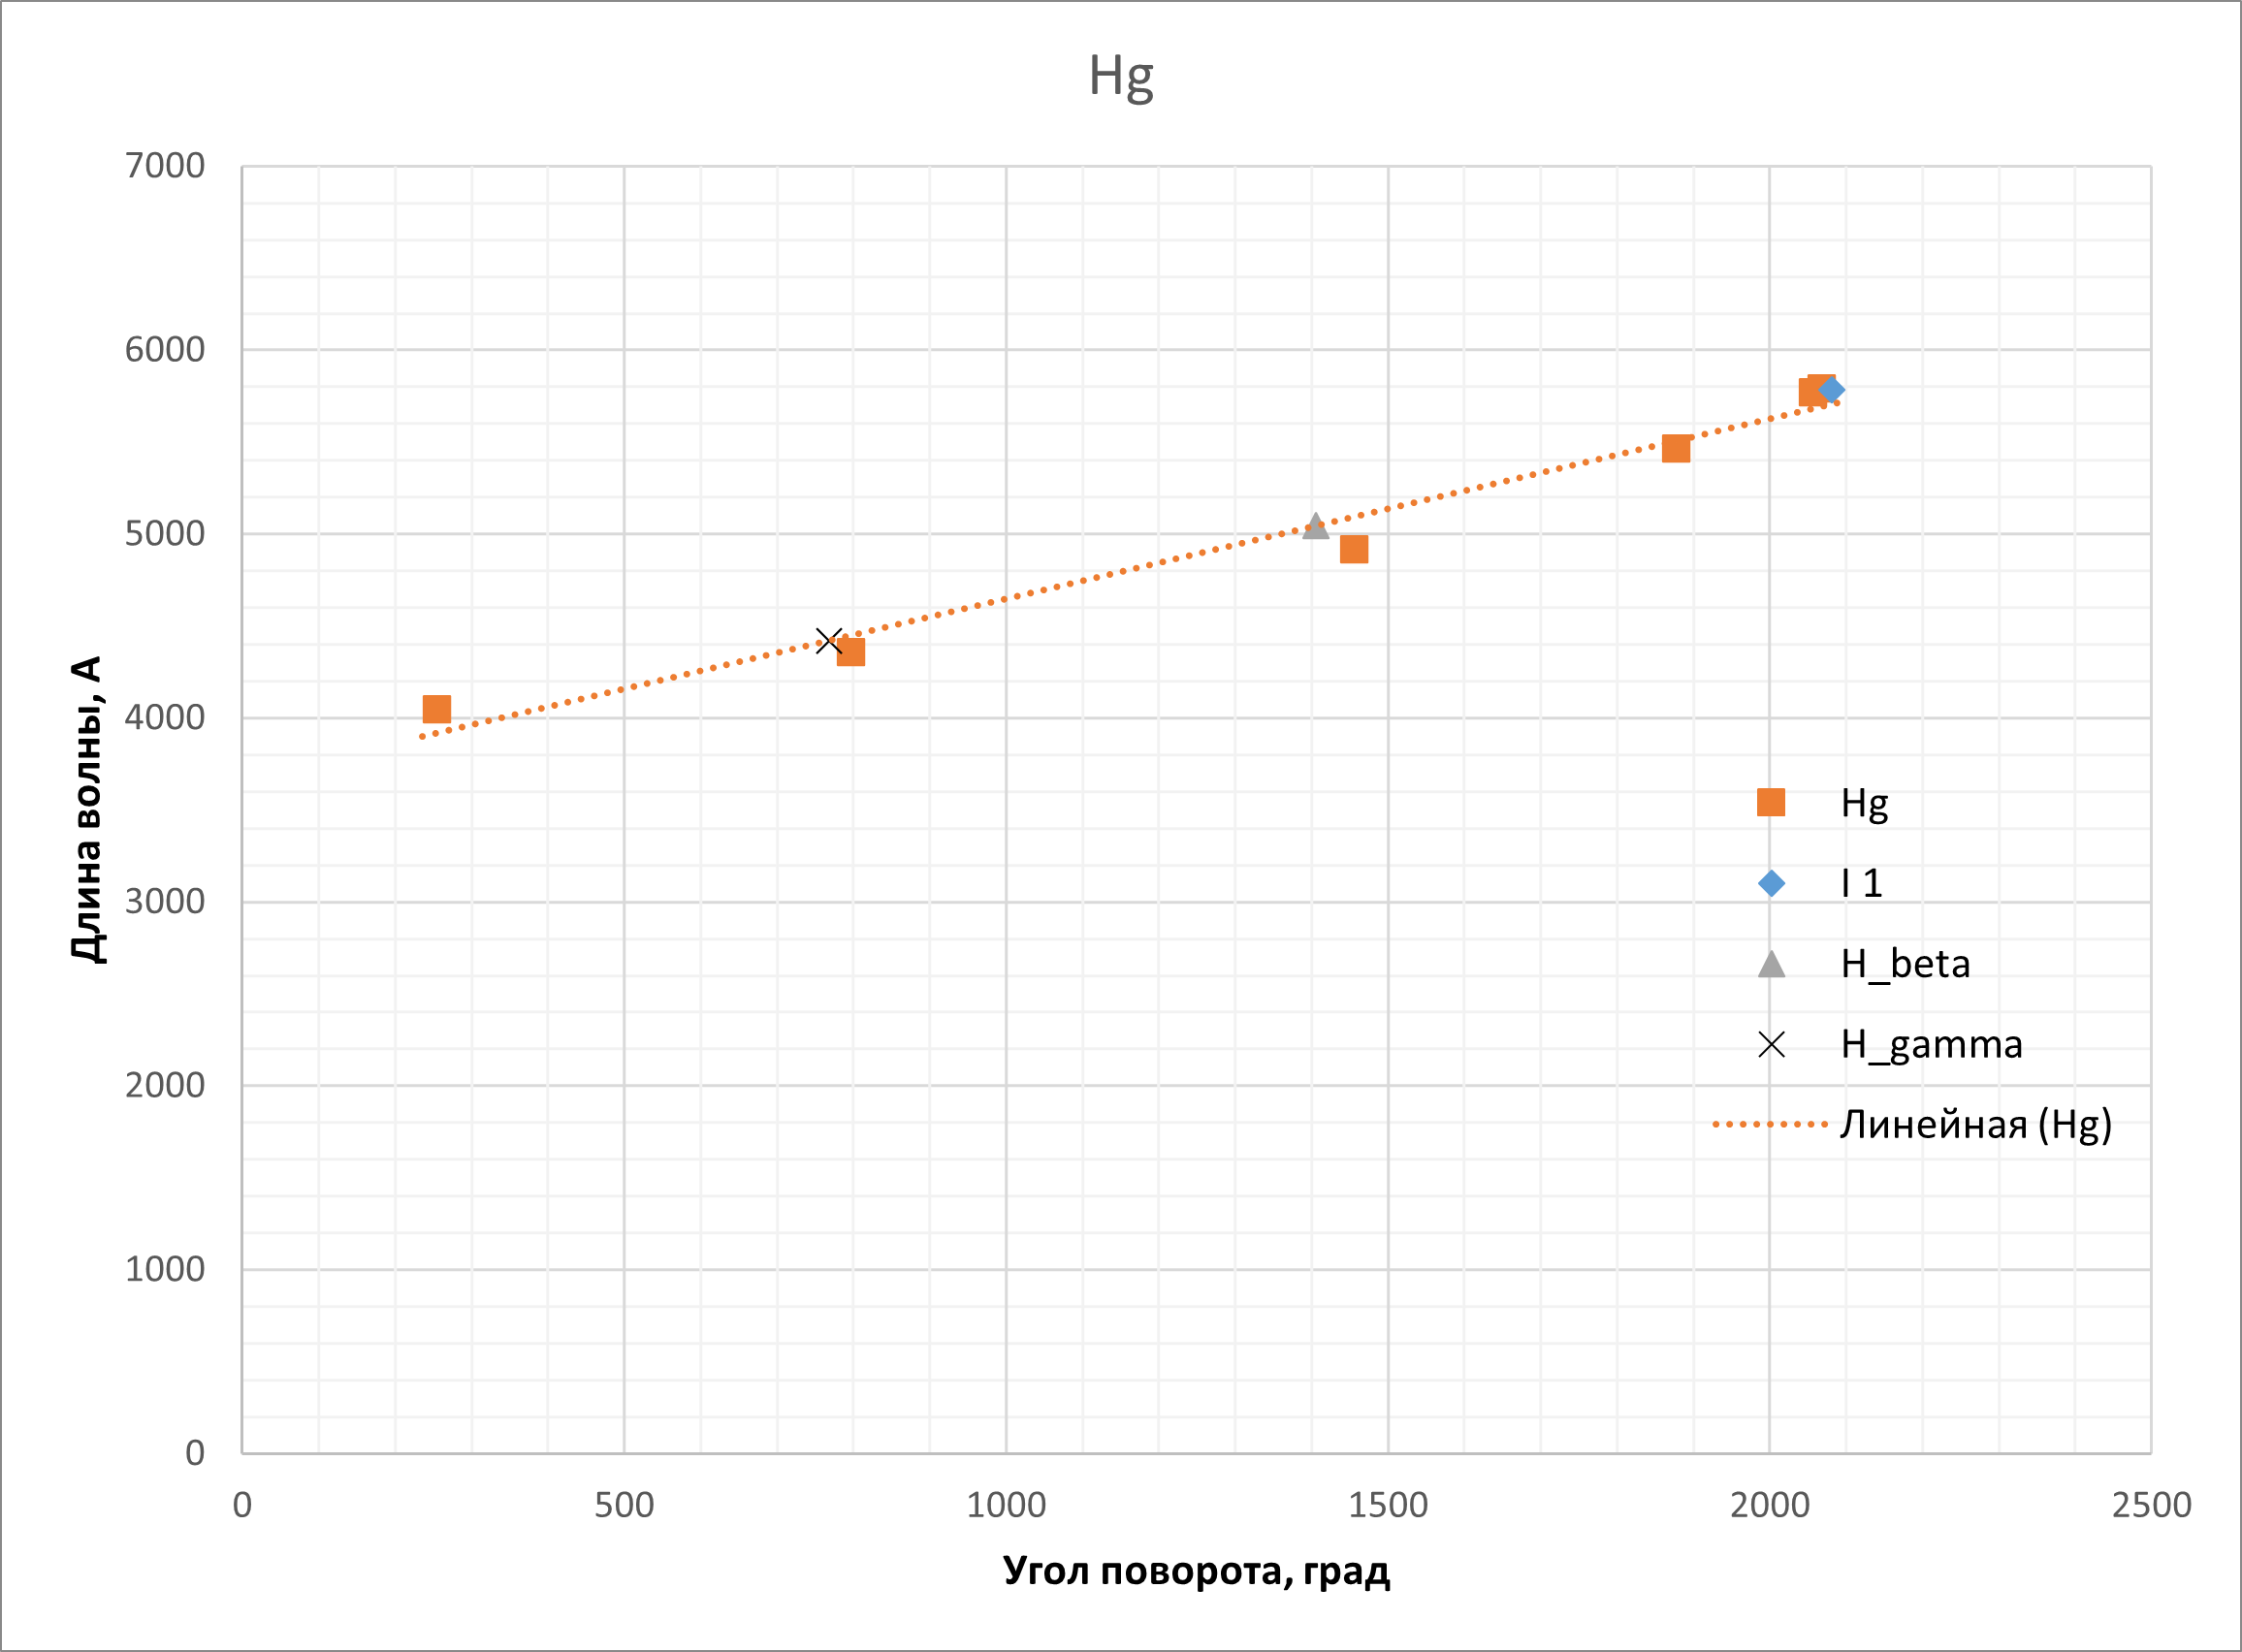
\includegraphics[width=0.7\textwidth]{img/HgPlot.png}
    \caption{Калибровка на Hg}
    \label{fig:Hg}
\end{figure}

\subsection{Спектр атомарного водорода}
Далее были измерены координаты (в единицах угла поворота барабана спектрометра) спектральных линий излучения атомарного водорода. Измерения проводились для первых трёх линий \textit{серии Бальмера} ($n=2$). Линии с номерами $m = 3,\,4,\,5$ обозначаются как $H_\alpha,\,H_\beta$ и $H_\gamma$ соответственно. При помощи рассчитанных ранее коэффициентов, получены оценки для длины волн в спектральном разложении водорода. Линию $H_\delta$ снять не удалось, так как она находится вне диапазона измерений УМ-2. Результаты и отклонения приведены в таблице ниже:
\begin{table}[!ht]
    \centering
    \begin{tabular}{|l|l|l|l|l|}
    \hline
        Линия & Результат, \r{A} & Табличное, \r{A} & Отклонение \\ \hline
        $H_\gamma$ & 4420 & 4341 & 1,8\% \\ \hline
        $H_\beta$ & 5044 & 4862 & 4\% \\ \hline
        $H_\alpha$ & 6546 & 6563 & 0,3\% \\ \hline
    \end{tabular}
\end{table}

Результаты укладываются в оценку погрешности. Отношение длин волн соответствует формуле сериальной закономерности \eqref{hydrogen}. Найдём значение постоянной Ридберга из полученных результатов:
\begin{table}[h]
    \centering
    \begin{tabular}{|c|c|c|c|c|} \hline
        Эксперимент & $H_\alpha$ & $H_\beta$ & $H_\gamma$ & Среднее \\ \hline
        $R$, см$^{-1}$ & 109990,8 & 105736,2 & 107735,3 & 107820,8 \\ \hline
        Отклонение от табличного, \% & 0,3 & 3,6 & 1,8 & 1,7 \\ \hline
    \end{tabular}
\end{table}
Относительные погрешности определения $R$ при расчёте из значений $\lambda$ совпадают с погрешностями определения $\lambda$ (т.\,к. $Z,\,n,\,m$~--- константы). Погрешность определения среднего значения:
\begin{equation}
\Delta_{\bar{R}} = \frac{1}{3}\sqrt{\sum\limits_{i=1}^3(R_i - \bar{R})} = 1468,3 \text{см}^{-1} = 0,013\bar{R}.
\end{equation}

\subsection{Спектр поглощения йода}
Аналогично предыдущему пункту были измерены длины волн, соответствующие энергетическим уровням $h\nu_{1,0},$ $h\nu_{1,5}$ и $h\nu_\text{гр}$. Результаты измерений представлены.
% Результаты измерений представлены в таблице \ref{tab:iodine}.
% \begin{table}[h]
%     \label{tab:iodine}
%     \centering
%     \begin{tabular}{|c|c|c|c|} \hline
%         Энергетический уровень & $h\nu_{1,0}$ & $h\nu_{1,5}$ & $h\nu_\text{гр}$ \\ \hline
%         $\lambda$, \r{A} & 5817 & 5622 & 4950 \\ \hline
%         $h\nu$, эВ & 2,14 & 2,21 & 2,51 \\ \hline
%     \end{tabular}
%     \caption{Результаты измерения для энергетических уровней йода}
% \end{table}
Так как $h$ и скорость света $c$~--- константы, то относительные погрешности определения $\lambda$ и $h\nu$ совпадают.

Оценку погрешностей расчета энергии колебательного кванта возбуждённого состояния молекулы йода можно по следующей формуле:
$$\Delta (h\nu_2) = \frac{1}{5} \sqrt{\Delta (h\nu_{1,5})^2 + \Delta (h\nu_{1,0})^2}.$$
Оценим погрешность измерения частоты:
$$\Delta(\nu) = \nu \frac{\Delta(\lambda)}{\lambda} \approx \nu \cdot 0.01$$
Итого, получаем оценку:
$$\Delta{\nu_{1,5}} \approx 0.03 \text{эВ} = \Delta (h\nu_{1,0}),$$
$$\Delta (h\nu_{\text{гр}}) \approx 0.04 \text{эВ},$$
$$\Delta (h\nu_2) \approx 0.005 \text{эВ}.$$
Таким образом, энергии уровней йода представлены в таблице \ref{tab:iodine1}.
\begin{table}[h]
    \label{tab:iodine1}
    \centering
    \begin{tabular}{|c|c|c|c|} \hline
        Энергетический уровень & $h\nu_{1,0}$ & $h\nu_{1,5}$ & $h\nu_\text{гр}$ \\ \hline
        $\lambda$, \r{A} & 5817 & 5622 & 4950 \\ \hline
        $h\nu$, эВ & 2,14 & 2,21 & 2,51 \\ \hline
        $\Delta (h\nu)$, эВ & 0.03 & 0.03 & 0.04 \\ \hline
    \end{tabular}
    \caption{Результаты для энергетических уровней йода}
\end{table}

С использованием табличных величин $h\nu_1 = 0,027$ эВ и $E_a = 0,94$ эВ по формулам \eqref{iodine1}-\eqref{iodine3} найдены следующие величины:
\begin{itemize}
    \item $h\nu_2 = (h\nu_{1,\,5} - h\nu_{1,\,0})/5 = 0,014\pm0,005$ эВ;
    \item $h\nu_\text{эл} = h\nu_{1,\,0} - \frac{1}{2}h\nu_2 + \frac{3}{2}h\nu_1 = 2,17\pm0,20$ эВ;
    \item $D_1 = h\nu_\text{гр} - E_a = 1,57\pm0,10$ эВ;
    \item $D_2 = h\nu_\text{гр} - h\nu_\text{эл} = 0,34\pm0,20$ эВ.
\end{itemize}

\section{Выводы}
В данной работе нам удалось пронаблюдать спектры излучения атомарных газов и спектр поглощения паров йода. Качественно все полученные результаты подтверждают предложенные теоретические модели. С достаточно большой точностью удалось определить постоянную Ридберга в опытах с атомарным водородом. Результаты в опыте с парами йода менее точны из-за плохой различимости спектральных линий в молекулярном спектре поглощения, а также из-за приблизительности используемой модели.